\documentclass{article}
\usepackage[utf8]{inputenc}

%Package enabling roman numerals in lists
\usepackage{enumitem}

%Package enabling dashed lines
\usepackage{arydshln}

%Package to show images
\usepackage{graphicx}
\graphicspath{ {./images/} }

%Package to display requirements as in SRS
\usepackage{tabularx}

\title{Architecture Notebook}

\author{Jonas Malm}
\date{October 2020\\---\\Version 0.4.4}

\begin{document}

\maketitle
\clearpage

\begin{table}
\section*{Version history}
\centering
\begin{tabular}{|l|l|l|l|}
\hline
Version & Date & Author & Description \\ \hline
0.1 & 2020-10-15 & Jonas Malm & Creation of document\\ 
0.2 & 2020-10-16 & Jonas Malm & Added architectural goals, finished ASRs\\
0.2.1 & 2020-11-02 & Jonas Malm & Added architectural constrains\\ 
0.3 & 2020-11-02 & Jonas Malm & Added architectural decisions\\
0.3.1 & 2020-11-04 & Jonas Malm & Refined decisions and ASRs\\
0.4 & 2020-11-04 & Jonas Malm & Added key abstractions and started layers\\
0.4.1 & 2020-11-05 & Jonas Malm & Wrote detailed layers\\
0.4.2 & 2020-11-09 & Jonas Malm & Added a glossary\\
0.4.3 & 2020-11-09 & Jonas Malm & Mades revisions based on feedback from Gustaf Eriksson\\
0.4.4 & 2020-11-09 & Jonas Malm & Re-wrote ASR to facilitate traceability\\

\hline
\end{tabular}
\end{table}
\textbf{TODO:}
\begin{enumerate}[label=(\roman*)]
\item  Improve section 5
\item  Write section 6
\item Add user cases?
\item Update ASRs when requirements are re-numbered
\item Populate appendix
\end{enumerate}


\clearpage

\tableofcontents
\clearpage

\section{Introduction}
\subsection{Purpose}
This document describes the software architecture of the system. Furthermore it describes the software modules that will be built and incorporated into the system, and delivers an overview of their function as well as an description of how they will support the project's goals.

\subsection{Definitions, acronyms and abbreviations}
\begin{description}
\item [EHR] An \emph{Electronic Health Record} is a record containing patient health data in an electronic form.
\item [OpenEHR] is a collection of open industry specifications, models and software for e-health.
\item [HCU] 
\item [OAuth] is an open standard for authorization delegation. It allows a service owner to allow third-party server access without sharing credentials, instead using access tokens. 
\item [AQL] The \emph{Archetype Query Language} is a declarative query language developed to search and retrieve data in archetype-based repositories, such as an OpenEHR-database.
\end{description}

\subsection{Goal of the project}
The key goal of HeartByte's product is to provide health care providers an easy-to-use system to monitor and care for a large group of patient with limited resources. Thus the architecture of this software contains modules that enable health care providers to gain an overview over a large group of patient while identifying key patients through autonomous classification and manual filtration and sorting, as well as supporting components.

\subsection{Architectural goals}
The goal of the architecture is to reach the project goal while fulfilling a few software specific goals. The customer has expressed a wish that the software be designed and build in accordance to the aspects below.

\subsubsection{Achieving high modularity with pre-built components}
The customer, Region Östergötland, wants to be able to combine parts from different systems together. In order for it to be possible to combine parts of HeartByte's software with parts from other systems, the software needs to be designed in a way so it maintains a high degree of modularity and a high degree of cohesion within modules. Otherwise combining functionality from HeartByte's software with other systems would be very difficult. Using pre-built, standardized components further enables this, since they are easily replaced and modular by definition.

\subsubsection{Ensuring integration with existing systems is easy}
In order to facilitate a simple integration process into existing systems the architecture needs to take existing systems into consideration. This includes loading and storing patient data in the same format as existing systems, loading and storing care giver data in the same format as existing systems and using the same kind of authentication method.

\subsubsection{Creating software independent of OS and platform}
Furthermore, the customer wants a system that can be used from different operating systems as well as platforms. Some care givers might use tablets running iOS while others use Android and others still use a computer or even a smartphone. In conclusion it is important for the customer that the system can be accessed and used from a multitude of OSs and platforms, which will have implications on the architecture and the choice of stack. 



\subsection{Architectural constraints}
Due to the nature of the project, there are several constraints which have to be considered. Most importantly, the time frame and the skills of the development team.

\subsubsection{Time constraint}
According the the project plan, the project is to be finished in about three months. The first month, iteration 0 and 1, is spent setting up an organizational structure, communicating with the customer to elicit needs and creating requirements and then one week of education for the development team. Then there are two weeks of developing in iteration 2, two weeks in iteration 3 and one week in iteration 4. 
Thus there are only five weeks where the system is to be developed. If the project is to be completed on time, these five weeks will have to be used effectively. The architecture of the system will have to reflect this and thus focus on creating the modules that add the most value to the customer, while using pre-built components as much as possible.

\subsubsection{Skill constraint}
Since there is only one week for educating the development team, the choice of stack will have to reflect this and try to leverage existing knowledge over creating new. According to the skill set study by \emph{Configuration Manager Sam Anlér}, the team is proficient in these languages:

\begin{table}[h]
\centering
\begin{tabular}{|l|l|l|}
\hline
Language & Number of proficient users & Share of team \\ \hline
Java & 23 & 88\% \\
HTML & 20 & 77\% \\ 
JavaScript & 18 & 69\% \\ 
SQL & 18 & 69\% \\ 
Python & 15 & 58\% \\ 
\hline
\end{tabular}
\end{table}



\subsection{Assumptions and dependencies}
\subsubsection{Assumptions}
\begin{enumerate}[label=(\roman*)]
\item The system will not be used on mobile devices, thus platform and OS independence applies only to computers and tablets 
\item The customer uses a openEHR system to store EHRs, and the same templates as 
\item The rules used in the rule engine are set by the HCUs admin and not by HeartByte. HeartByte thus cannot take responsibility over if scientifically correct rules are applied, only that the patients are prioritized according to them.
\end{enumerate}
\subsection{Dependencies}


\section{Architecturally significant requirements}
Listed below are the Architecturally significant requirements (ARSs), the requirements most central to the architectural design. 

\subsection{Patient views}
\begin{tabularx}{\linewidth}{| l | X |}
 \hline
 \textbf{ID:} & FR007  \\ 
 \hline
 \textbf{Statement:} & The user shall be able to shift between a "patient view" where many patients are shown and a "overview view" where only one patient are shown. \\
 \hline
\end{tabularx}
\\ \\

Below, ASRs about these two views will be presented. The view displaying many patients will we refere

\subsubsection{Patient overview}
\begin{tabularx}{\linewidth}{| l | X |}
 \hline
 \textbf{ID:} & FR009  \\ 
 \hline
 \textbf{Statement:} & The admin shall be able to specify the variables that affects the health prioritization. The system shall provide the possibility to specify different variables for different health care units. 
 \\ 
 \hline
 
 \textbf{ID:} & FR004  \\ 
 \hline
 \textbf{Statement:} & The system shall display all patients in preferred order to a user who sort patients by [age, alert-level, measurements, health care unit, team, disease and patients’conditions]. \\ 
 \hline
 
 \textbf{ID:} & FR003  \\ 
 \hline
 \textbf{Statement:} & The system shall display all matching patients to a user who filter patients by [age, alert-level, measurements, health care unit, team, disease and patients’conditions]. \\ 
 \hline

 \textbf{ID:} & FR011  \\ 
 \hline
 \textbf{Statement:} & The admin shall be able to customize and save different views of the system. (e.g. a predefined view over diabetes patients who are over 30 years)
  \\ 
 \hline
\end{tabularx}
\\ \\

The requirements state that the software shall have an overview of patients where a health care provider can:
\begin{enumerate}[label=(\roman*)]
\item prioritize patients assisted by a module implementing care unit-specific triage rules,
\item sort patients,
\item filter patients based on multiple criteria,
\item save and load these filter views for later use.
\end{enumerate}
Thus a rule engine will be implemented that loads rule sets created by an admin as well as a database storing custom filter views and custom rules.


\subsubsection{Patient view}

\begin{tabularx}{\linewidth}{| l | X |}
 \hline
 \textbf{ID:} & FR026  \\ 
 \hline
 \textbf{Statement:} & In the view of a patient user shall be able to see personal information (gender, age occupation, social security number) 
 \\ 

 \hline
 \textbf{ID:} & FR043  \\ 
 \hline
 \textbf{Statement:} & In the overview of a patient the user shall at the top of the view be presented with the patient’s current medication(s).
 \\ 
 \hline

 \hline
 \textbf{ID:} & FR044  \\ 
 \hline
 \textbf{Statement:} & In the overview of a patient the user shall at the bottom of the view be presented with responsible healthcare provider(s) and associated hospital or clinic.
 \\ 
 \hline
\end{tabularx}
\\ \\

The requirements state that detailed information about a patient from his or her EHR is to be displayed in a dedicated view for the specific patient. This information includes current medications, next of kin, health data as well as a calendar visualizing upcoming events for the patient.

\subsubsection{Format}
\begin{tabularx}{\linewidth}{| l | X |}
 \hline
 \textbf{ID:} & NFR013  \\ 
 \hline
 \textbf{Statement:} & The system shall enable use of openEHR platforms as storage backend for EHR content (e.g. measurements, content from forms filled out by the patient and care plan).
 \\ 
 \hline
\end{tabularx}
\\ \\

The requirements further stipulate that all patient \emph{Electronic Health Records}, EHRs, have to be stored and loaded from databases in accordance with the \emph{openEHR open standard specification}. This is furthermore of great importance to the customer, since they cannot integrate the software with its existing software and servers without the key requirement being fulfilled.

\subsubsection{Patient data and access}

\begin{tabularx}{\linewidth}{| l | X |}
 \hline
 \textbf{ID:} & FR038  \\ 
 \hline
 \textbf{Statement:} & The user shall only get access to the data if the user chooses to access it
  \\ 
 \hline

 \textbf{ID:} & FR006  \\ 
 \hline
 \textbf{Statement:} & The system shall notify the user if they tries to access patient data that they don't have authority to view.\\ 
 \hline

 \textbf{ID:} & FR008  \\ 
 \hline
 \textbf{Statement:} & The system shall log which users who viewing which patients. These activities shall be saved in a log file.
\\ 
 \hline

 \textbf{ID:} & NFR002  \\ 
 \hline
 \textbf{Statement:} & OAuth shall be used for login and authentication.
 \\ 
 \hline
\end{tabularx}
\\ \\

Health records are highly regulated and one important aspect is who is allowed to see what patient data. Thus the requirements state that the software shall save logs when a user accesses EHRs. The requirements also state that the users have to authenticate themselves using OAuth. 
Thus the following modules need to be implemented:

\begin{enumerate}[label=(\roman*)]
\item A database storing access logs
\item A database storing which Health Care Unit (HCU) a user belongs to, so it can be determined if a user has authority to access
\item An authentication system using OAuth
\end{enumerate}



\section{Architectural decisions}
Below are the most important architectural decisions listed, stemming from the architectural goals, the architectural constraints and the ASRs.

\subsection{Using a back end}
In order to accommodate the two database mentioned in the \emph{Access ASR}, a back end containing the access log and personnel databases needs to be implemented. This is because in order to ensure that EHRs are not served to unauthorized clients, the calls to the actual EHR Database will have to go through a server that logs access. Doing this client side would not be as secure since a modified client could simply bypass the logging or not validate access levels through the personnel database.

\subsection{Choice of front end stack}
The front end will be developed using the JavaScript framework ReactJS. This is due to a few reasons:

\begin{enumerate}[label=(\roman*)]
\item By building a web app and using React, \emph{platform and OS independence} is enabled.
\item Due to the skill constraint, we want to leverage existing knowledge. The team is proficient in JavaScript and \emph{React is a JavaScript framework}.
\item Due to the time constraint, we need a language that is \emph{quick to learn and simple to use}. This holds true for React, which due to its wide spread use has many tutorials and good documentation.
\item One of the architectural goals is to achieve \emph{high modularity through reusable components}. React facilities this through allowing developers to split the UI into independent components and there are many free open-source components because of the popularity of the framework enabling quick development.
\end{enumerate}

\subsection{Choice of back end stack}
Due to the time and skill constraints, this back end and the databases would ideally leverage existing knowledge in the team. The back end will be developed in Python, using the web framework Flask for the server and the framework SQL Alchemy for the databases. The rationale behind these decisions is explained below.

\subsubsection{Python}
Python is a language that is easy to work with and easy to read; is easy to read, very popular as a back end language which ensures good help and has many web application frameworks. Since a majority of the team already are familiar with Python and the reasons listed above it is a good choice for back end. 
\subsubsection{Flask}
The Flask web framework is easy to use, flexible and allows for unit testing through integrated support and a quick debugger. Furthermore some members of the team are already familiar with Flask, so it is a good choice as web framework.
\subsubsection{SQL Alchemy}
Since members are experienced with SQL and the back end will be developed in Python, a logical step is using the SQL Alchemy framework in order to make the database development faster. There are also members of the team that are familiar with this framework.

\subsection{Using EhrScape}
As specified in the ASRs, the patient EHRs must be stored using the openEHR standard. Due to the time constraint and the skill constraint, the project does not have time to either train developers or to develop a server storing EHRs in accordance to the openEHR standard. In order to accommodate this requirement the project will instead use EhrScape, a health data platform. The platform contains tools for easy handling of clinical models, health data queries and vendor independent data storage. This is accessed through an API and data is stored on EhrScape's EHR server.



\section{Key abstractions}
The key abstractions of the system is the front end, the back end and the EHR Database. The front end is what the user interacts with and the services supporting this. The back end contains the two databases and functionality to get data from these databases. The EHR Database is the external database storing the patient's EHR.

\begin{figure}[h]
    \centering
    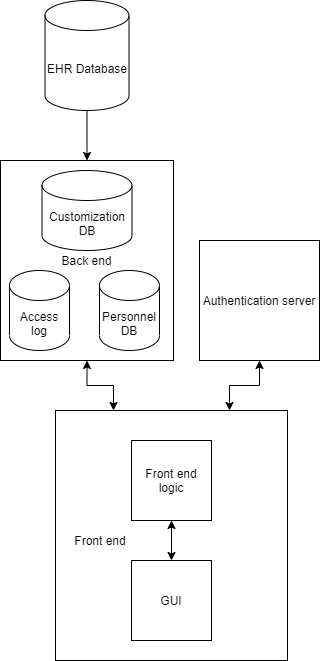
\includegraphics[scale = 0.5]{key-abstraction}
    \caption{The system and its key abstractions}
    \label{fig:key-abstractions}
\end{figure}


\subsection{Front end}
The main functionality of the front end is to create a way for the user to interact with and visualize patient data. The user will do this through the GUI, and the GUI will then communicate with the front end logic to enable the user to filter, sort and group patients. 

\subsection{Back end}
The back end serves the purpose set out in the in the ASRs and the architectural decisions. The back end will handle calls to the EHR Database and ensure that if a user accesses patients outside his or her patient group this is logged. The back end will also handle calls to the personnel database as well as storing the customization of the interface, patient views and rules for the rule engine.

\subsection{EHR Database}
The EHR Database is the database that store the patient EHRs. It will also store any custom AQL queries that are created to access the patient EHRs and templates used to store EHR data.


\section{Architectural views}
\subsection{System layers}
This section will describe components of the system in a detailed way through four layers: the GUI, the Front End Logic, the HeartByte Server and the EhrScape Server. The direction of the arrows indicate the direction of data flow.

\begin{figure}[h]
    \centering
    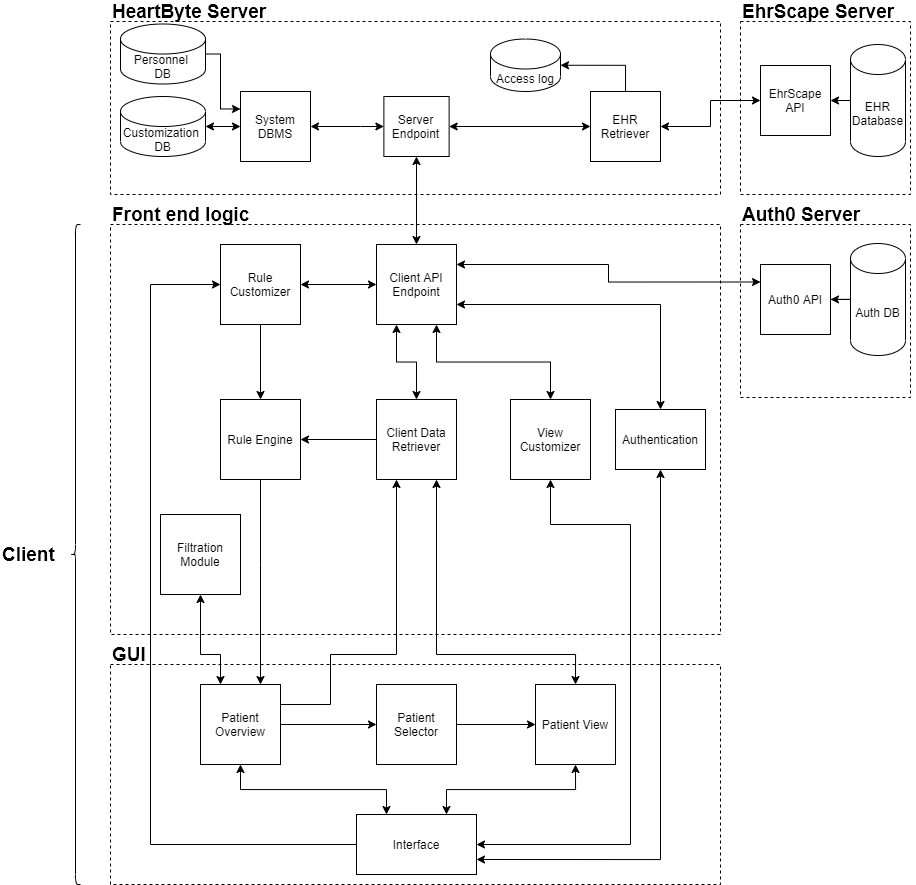
\includegraphics[scale = 0.3]{box-and-line}
    \caption{A box and line diagram illustrating layers of the system and its submodules}
    \label{fig:execution-view}
\end{figure}

As seen in Figure \ref{fig:execution-view} the front end and back end interface will utilize the facade design pattern, so coupling and modularity is ensured. Below, the modules in the figure will be described by layer.

\subsubsection{GUI Layer}
The GUI consists of four main modules. The Interface is what the user will interact with and what will display the web app. From the Interface the user can access the Patient Overview, displaying many patients, and through the Patient Selector select a specific patient to be displayed in the Patient View. 

The Interface also allows a user to log in and for superusers, to customize the rules applied in the Rule Engine through the Rule Customizer and how components in the Interface are displayed through the View Customizer.

\subsubsection{Front End Logic Layer}
The Front End Logic contains the "middleware" interacting with the HeartByte Server and the GUI to deliver data to the GUI. The most central module is the Client Data Retriever. This module will handle calls from Patient Overview to get general data about a group of patients and calls from Patient View to get detailed data about a specific patient. 

When Patient Overview makes a call to this module, the servers response is passed to the Rule Engine for classification of how critical the patients health status is. Then the classified data is passed through the Filtration Module and then to the Patient Overview to be displayed. The Patient Overview can also make calls directly to the Filtration Module to change the filters applied to the data already retrieved. When the Patient View makes calls to the Client Data Retriever, the results returned from the server are passed directly to the Patient View.

This layer also contains the modules used for authentication as well as the customization a superuser can do. To customize classification rules, the Interface calls the Rule Customizer which in turn loads or stores rules in the Customization Database. The View Customizer works in the same fashion. The Authentication module will make a call to the Personnel Database to determine what role the user has, and thus what information should be displayed.

\subsubsection{HeartByte Server Layer}
The HeartByte Server contains the databases specific to the system and the functionality to retrieve EHRs. The System Database Management allows for storing and loading data in the Personnel Database and the Customization Database. These databases contain data about custom rules and views for specific HCUs and personnel data, respectively.

The EHR Retriever is the module responsible for loading data from EHRs. This module will recieve a call about what data to retrieve, make a call to the EhrScape Server to retrieve the requested data and return the data through the Server Endpoint. The EHR Retriever will also make a call to the Personnel Database in order to check if the user requesting the EHR data works at one of the HCUs responsible for the patient. If this is not the case, this will be added to the log entry in the Access Log database.

\subsubsection{EhrScape Server Layer}
This layer is a database stored on an external server, which is accessed using the EhrScape API. The API is queried using stored custom Archetype Query Language (AQL) queries as well as using its REST API. Since this is the openEHR database query language it is easy to substitute this layer with another openEHR server in the future.


\section{The system in the future}
\textbf{TODO:} 
This is only a stub, to be completed in the future
\subsection{Scaleability}
EHR Retriever & changing the database to live. Rule engine on large scale? Filtration on large sets? Personnel database and the scope tokens?
\subsection{Support}
\subsection{Maintaining}
Changing database. Leaving openEHR? 
\subsection{Future development}
Due to the time constraint, some functionality was cut. In this section these modules will be described in more general terms. As this section is not finished and the final functionality of the product is not yet set, what is listed below might be implemented.
\subsubsection{Trend analysis}
\subsubsection{Calendars}
\subsubsection{Notifications}

\section{Appendix}
\textbf{TODO:} Populate
\subsubsection{OpenEHR Templates}


\end{document}
